
\section{Introducción}

En esta sección se aborda el proceso de transmisión de información y se analizan las operaciones biológicas que hacen posibles los cómputos en el cerebro. Para empezar a modelar una red neuronal se detallará primero la dinámica de los disparos neuronales.

Recordando los conceptos abordados en el  capítulo  anterior, las neuronas son células especializadas del sistema nervioso central que se comunican mediante señales tanto eléctricas como químicas.  Son células con núcleo, axón y dendritas capaces de transferir impulsos eléctricos. La transmisión de un pulso eléctrico se lleva a cabo desde el soma a través de sus membranas, pasando por los nodos de Ranvier a lo largo del axón, hasta la terminal del axón en los botones sinápticos. Las neuronas hacen sinapsis  permitiendo que el pulso llegue a las dendritas de la neurona postinanáptica, mediante canales iónicos. \parencite{neurona_A_cerebro}

El pulso eléctrico que se desplazo desde el cono axónico de la neurona presináptica hasta la neurona postsináptica, se genera por la diferencia de potencial existente entre el interior y el exterior de la neurona, el cual resulta de las varias concentraciones de iones en ambos lados de la membrana plasmática. Los estados potenciales neuronales presentes en la membrana plasmática del axón se distinguen en los siguientes \parencite{HH}:

\begin{itemize}
\item \textbf{Potencial de reposo:} Se refiere a la diferencia de cargas eléctricas a través de la membrana celular cuando no hay una señal nerviosa en curso. La membrana está polarizada a -70 mV, lo que significa que tiene una carga positiva en el exterior (por la presencia de iones de sodio, Na+) y una carga negativa en el interior debido a iones como el cloruro (Cl-) y proteínas. En este estado, la membrana no transmite señales nerviosas. Ver la figura \fref{fig:MembranaP} lado derecho.

\item \textbf{Potencial de acción o membrana:}  Se produce cuando un estímulo alcanza un nivel umbral de 55 mV. Este evento despolariza la membrana, lo que significa que cambia rápidamente su polaridad de negativa a positiva. Esto ocurre porque se abren canales de iones de sodio (Na+) y potasio (K+), permitiendo el flujo de estos iones a través de la membrana, ver la figura \fref{fig:MembranaP} lado izquierdo. Este cambio rápido en la polaridad de la membrana es lo que impulsa el avance de la señal nerviosa. Las etapas del potencial de acción está representado en la figura \fref{fig:graficaP}
\end{itemize}


\begin{figure}[h]
 \centering
 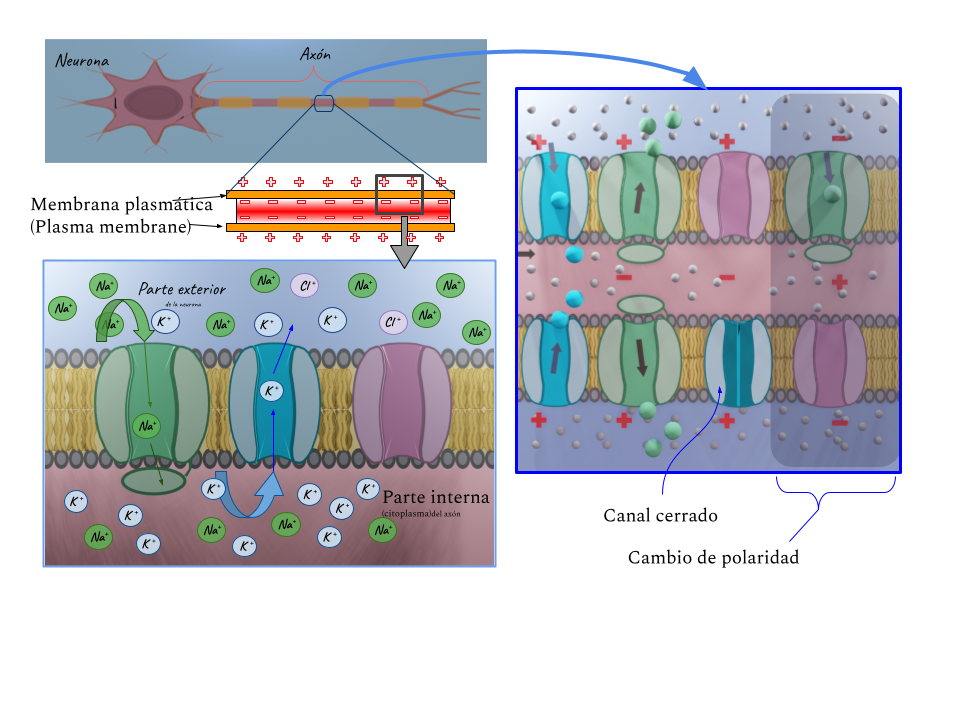
\includegraphics[scale=0.5]{../Figuras/MembranaP.png}
 \caption{Representación de la membrana axónica en potencial de reposo en la parte inferior izquierda, y en la parte derecha con un estímulo que genera el cambio de polaridad en la misma, así como el cierre de canales y paso de iones.}
 \label{fig:MembranaP}
\end{figure}

\begin{figure}[h]
 \centering
 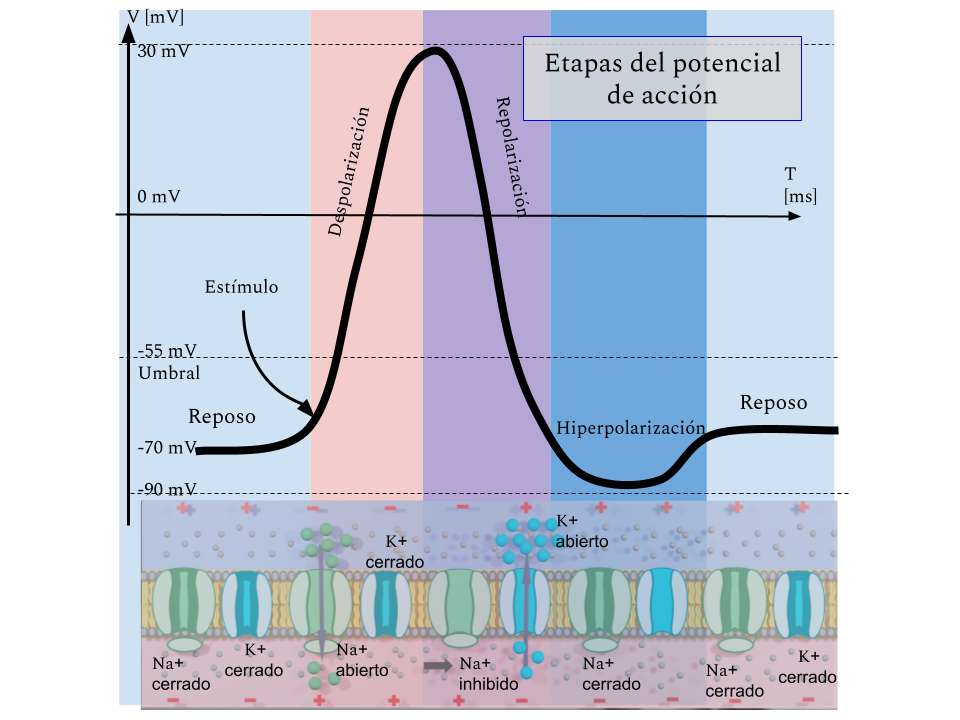
\includegraphics[scale=0.5]{../Figuras/Grafica.png}
 \caption{Representación gráfica de la respuesta de los canales iónicos de sodio (Na+ en verde) y potasio (K+ en azul) ante un estímulo de voltaje, dando como resultado un potencial de acción que viajará a lo largo de todo el axón.}
 \label{fig:graficaP}
\end{figure}

Los pioneros en el estudio del potencial de acción y elaboración de un modelo para la unión sináptica eléctrica fueron Alan Lloyd Hodgkin y Andrew Fielding Huxley alrededor de 1952. Este modelo matemático, intentaba esclarecer los procesos neuronales, surgió a partir de investigaciones experimentales  \footnote{El texto original de este experimento se puede encontrar en la siguiente url: \url{ https://physoc.onlinelibrary.wiley.com/doi/pdf/10.1113/jphysiol.1952.sp004764}}.

Estos científicos llevaron a cabo sus estudios utilizando un calamar gigante, un animal que puede alcanzar hasta 4 metros de longitud y posee un axón a proporción, que se extiende casi a lo largo de la mitad del cuerpo del calamar y tiene un grosor de medio milímetro, en comparación con el tamaño estándar del axón de una neurona, que oscila entre 1 y 20 micrómetros. 
El axón del calamar gigante es tan grande que les permitió introducir dispositivos para medir el voltaje, es decir, la diferencia de potencial entre el interior y exterior de la neurona. Con estas mediciones experimentales, lograron determinar las dinámicas de las cargas eléctricas tanto en el interior como en el exterior de la neurona, lo que facilitó el estudio de la transferencia de electricidad durante la activación de un impulso nervioso.
 

\section{Membrana y canal}

Durante las observaciones del flujo de corrientes eléctricas el sistema parecía comportarse como un circuito eléctrico, donde la membrana actuaba como un componente poroso que \textit{funciona como un capacitor}, almacenando ligeramente las cargas cuando intentan pasar de un lado a otro. Además esta membrana tiene la cualidad de permitir el paso selectivo de iones en ciertos momentos, es decir es una estructura \textit{semipermeable} que se representa con \textit{resistencias variables}. Ver Figura \ref{fig:ModelHh}.

Los canales de iones permiten o bloquean el flujo de iones dependiendo de la diferencia de potencial que exista entre el interior y el exterior de la membrana y de su estado de reposo particular. Por tanto es necesario agregar los potenciales de reposo para cada canal al modelo, en la figura \ref{fig:circuito} se agregan.


\begin{figure}[h]
 \centering
 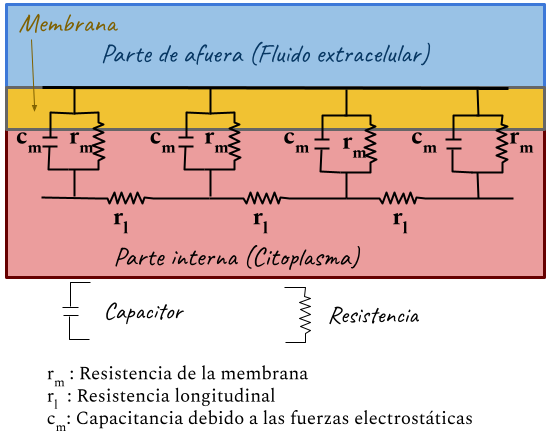
\includegraphics[scale=0.5]{../Figuras/ModeloHH.2}
 \caption{Un primer modelo de la membrana axónica modelada como circuito eléctrico.}
 \label{fig:ModelHh}
\end{figure}



\begin{figure}[h]
 \centering
 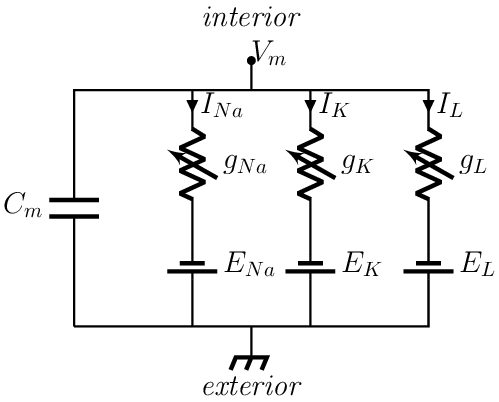
\includegraphics[scale=0.5]{../Figuras/circuito.png}
 \caption{Modelo de la membrana axónica modelada como circuito eléctrico, con los distintos canales presentes y sus voltajes en reposo.}
 \label{fig:circuito}
\end{figure}

Los elementos necesarios para el modelo de la membrana son los siguientes:
\begin{itemize}
\item Potenciales eléctricos \emph{E ó  V}; Se mide en \emph{mV}.
    \begin{itemize}
     \item \emph{E\textsubscript{(Na,K,L)}} 
     Potencial de equilibrio o reposo para los iones de sodio (Na), potasio (K) y cloruro y de fuga (L). 
     \begin{itemize}
        \item E \textsubscript{Na}  \emph{50mV}
        \item E \textsubscript{Ca}  \emph{150mV}
        \item E \textsubscript{K}   \emph{- 80mV}
        \item E \textsubscript{Cl}  \emph{- 60mV}
        \end{itemize}

     \item \emph{V\textsubscript{m}} Potencial eléctrico de la membrana. 
     \end{itemize}

\item Corriente \emph{I}; Movimiento de cargas. Se mide en \emph{µA}.
    \begin{itemize}
     \item \emph{I\textsubscript{(Na,K,L)}} corriente entrante a los canales de Na, K o L.
     \end{itemize}

\item Resistencia \emph{R}; Medida de la oposición al movimiento de las partículas cargadas.
\item Capacitancia o capacidad eléctrica \emph{C} . Cantidad de energía eléctrica almacenada en un capacitor para una diferencia de potencial eléctrico dada.
    \begin{itemize}
     \item \emph{C\textsubscript{m}} la capacitancia de la membrana. 
     \end{itemize}

\item Conductancia \emph{g}; Inverso de la resistencia \( \dfrac{1}{R} \) , es decir, facilidad de transmisión de las partículas cargadas.
    \begin{itemize}
     \item \emph{g\textsubscript{(Na,K,L)}}  la conductancia del canal de sodio, potasio, cloro y fuga. 
     \end{itemize}

\end{itemize}

\section{Modelo de los canales de inoes}

En la figura \fref{fig:MembranaP} se puede ver la representación de membrana y sus lipidos, la carga es almacenada en la membrana por un breve periodo de tiempo, dando como resultado que la bicapa se comporte como un \textbf{capacitor}. Esta membrana también está con cierta resistencia al paso de corriente representado en el diagrama \ref{fig:circuito} \footnote{Otra explicación más detallada la podemos encontrar en \url{https://neurowiki.case.edu/wiki/Action_Potential_IV:_Hodgkin-Huxley_Equations_and_Other_Conductances}} 

La membrana de una neurona es modelada como un elemento de un circuito con capacitancia \emph{C\textsubscript{m}} y potencial \emph{V}, las corrientes que fluye a través de la bicapa lipídica están regidos por las siguientes ecuaciones:

\begin{equation}
  I_{m} = C_{m} \dfrac{dV_{m}}{dt}
  \label{eq:corrientesEnLaMembrana}
\end{equation}


\begin{equation}
  C_{m} \dfrac{dV_{m}}{dt} =  - g_{Na} m^3 h(V - E_{Na} ) - g_{K} n^4 (V - E_{K} ) - g_{L} (V - E_{L} ) + I_ext
  \label{eq:corrientesEnLaMembrana2}
\end{equation}

\begin{equation}
  \dfrac{1}{\gamma(T)}\dfrac{dn}{dt} =  \alpha_{n^\infty} (V)(1 - n) - \beta_{n} (V) n = \dfrac{n(V)-n(t)}{\tau_{n}(V)}
  \label{eq:corrientesEnLaMembrana3}
\end{equation}

\begin{equation}
  \dfrac{1}{\gamma(T)}\dfrac{dm}{dt} =  \alpha_{m} (V)(1 - m) - \beta_{m} (V) m = \dfrac{m^\infty(V)-m(t)}{\tau_{m}(V)}
  \label{eq:corrientesEnLaMembrana4}
\end{equation}

\begin{equation}
  \dfrac{1}{\gamma(T)}\dfrac{dh}{dt} =  \alpha_{h} (V)(1 - h) - \beta_{h} (V) h = \dfrac{h^\infty(V)-h(t)}{\tau_{h}(V)}
  \label{eq:corrientesEnLaMembrana5}
\end{equation}

La ecuación principal es \ref{eq:corrientesEnLaMembrana} que donde la corriente de la membrana está dada por su capacitancia con el cambio voltaje en la membrana respecto al tiempo.

Cada una de las partes del lado izquierdo de la ecuación \ref{eq:corrientesEnLaMembrana2} corresponde a las compuertas de los canales y la corriente de un estímulo escrictamente externo que pueda influir a la membrana.

De manera sencilla podemos notar al canal de potasio como una puerta hecha de cuatro subpuertas por donde los elementos pasan o no pasan, es decir tiene dos estados; activado o desactivado. El canal de sodio lo podemos notar como una puerta que está hecha de tres subpuertas que se pueden abrir y tiene aparte un tapón extra, que hace que aunque estas tres están abiertas bloquee toda la compuerta, es decir tiene tres estados; desactivado, activado, inactivo. Con esto podemos representar a las conductancias \textbf{g} como:

\begin{itemize}
 \item \(\dfrac{1}{R_{Na}} = g_{Na} * m ^3 * h \) donde \(g_{Na}\) es una constante que representa el valor de la conductancia máxima, \textbf{m} es la proporción de los canales de sodio abiertos (representa la concentración de sodio) y nos indica la activación (subpuertas abiertas) del canal, \textbf{h} es el “tapón” de la compuerta que puede impedir el paso de iones independientemente de las otras tres subpuertas, es decir la inactivación (compuerta bloqueada).
Los movimientos combinados de \textbf{m} y \textbf{h} son los que controlan la compuerta de sodio.
 \item \(\dfrac{1}{R_{K}} = g_{K} * n^4\) donde \(g_{K}\) es una constante que representa el valor de la conductancia máxima, \textbf{n} es la proporción de los canales de potasio abiertos (representa la concentración de potasio) y nos indica la activación del canal de potasio.
 \item \(g_{L}\) es una constante, de los canales por fuga, que representa la concentración de los demás iones que pasan por la membrana.
\end{itemize}

Las concentraciones de iones están dado por \emph{m}, \emph{n} y \emph{h}, que son variables de activación que describen la probabilidad de que los canales iónicos estén abiertos. Donde la ecuación \ref{eq:corrientesEnLaMembrana3} representa las subcompuertas del canal de potasio y las ecuaciones \ref{eq:corrientesEnLaMembrana4} y \ref{eq:corrientesEnLaMembrana5} representando las subpuertas al canal de sodio tomando en cuenta que tiene dos tipos de subpuertas.

Las expresiones de \(\alpha\) y \(\beta\) están dadas por las siguientes ecuaciones:

\begin{align*}
\alpha_{n}&=\dfrac{0.01(10-V)}{exp(\dfrac{10-V}{10})-1}           &  \beta_{n}&=0.125exp-\dfrac{V}{80}\\
\alpha_{m}&=\dfrac{0.01(25-V)}{exp(\dfrac{25-V}{10})-1}                    &  \beta_{m}&=4exp-\dfrac{V}{18}\\
\alpha_{h}&=\dfrac{0.07}{exp-(\dfrac{V}{20})}              &  \beta_{h}&=\dfrac{1}{1+exp\dfrac{30-V}{10}}
\end{align*}

Los factores \(\alpha\) y \(\beta\) se denominan como constantes de velocidad de transición. \(\alpha\) es el número de veces por segundo que se abre una puerta que está en estado cerrado, mientras que \(\beta\) es el número de veces por segundo que se cierra una puerta que está en estado abierto. Si la membrana tiene un la carga negativa, \(\alpha\) debe aumentar y \(\beta\) debe disminuir, cuando la membrana esté despolarizada.


\subsection{Las conductancias iónicas}
Nuestro objetivo aquí es encontrar ecuaciones que describan las conductancias con precisión razonable y lo suficientemente simples para el cálculo teórico de \emph{el potencial de acción} y \emph{el período refractario}. 

Si tomamos las ecuaciones diferenciales anteriores notamos que las soluciones tienen este tipo de forma \ref{fig:graficaX}:

\begin{figure}[h]
 \centering
 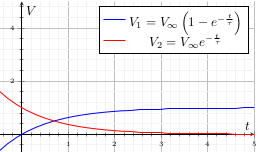
\includegraphics[scale=0.8]{../Figuras/solPulso1.png}
 \caption{Soluciones para el pulso.}
 \label{fig:graficaX}
\end{figure}


Donde si estamos aplicando una corriente externa lo que sucede es lo que estamos viendo en azul, un exponencial que va creciendo y que tiende hacia un cierto valor límite que sería de infinito. Si dejamos de aplicar la corriente externa entonces ahora tendremos un exponencial, pero que tiende hacia el cero y se va a estabilizar en cero, lo que vemos en rojo. 

\begin{figure}[h]
 \centering
 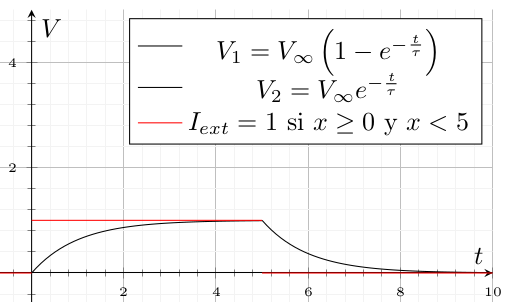
\includegraphics[scale=0.5]{../Figuras/solPulso2.png}
 \caption{Soluciones para el pulso escalón.}
 \label{fig:graficaX1}
\end{figure}

Simulando lo que hicieron Hodgkin y Huxley que fue al axón de repente darle un toque, siendo en el origen de la gráfica (que visualizamos en la figura \ref{fig:graficaX1}) la parte en la que le están dando el toque al axón, momentos antes estaba quieta la neurona de repente le aplican una cierta cantidad de electricidad y va a empezar a cambiar el comportamiento de los canales la porosidad de la membrana, vamos a ver que empieza a incrementarse la diferencia de potencial hasta que llegan a un nuevo equilibrio (alrededor de t = 3) y si siguieran dándole el toque en esa cantidad se quedaría ahí la neurona, ya no veríamos más cambios lo que va a suceder entonces es que, retiramos las pinzas (se le deja de dar el toque) y los canales otra vez van a empezar a regresar a la normalidad y vamos a ver un descenso en adelante.

Entonces hasta aquí ya tenemos la idea de cómo va a reaccionar la neurona ante cierto estímulo; sin embargo, esto que acabamos de ver en las gráficas sería como si tuviéramos un solo tipo de canal, ahora qué pasa si consideramos que tenemos diferentes tipos de canales pasando iones, en condiciones distintas. 
Aquí es donde va a importarnos el hecho de que existen diferentes tipos de canales con voltajes de equilibrio diferente. 
Retomando a los potenciales de Nerst \(E_{Na},E_{K},E_{L}\) notemos que están dados por:


\begin{equation}
    E = \dfrac{k_{B}T}{zq}\ln\dfrac{[adentro]}{[afuera]}
 \label{eq:diferenciaP}
\end{equation}

Estos potenciales están relacionados con las características termodinámicas, en la ecuación anterior \ref{eq:diferenciaP} \(k_{B}\) la constante de Boltzman, \(q\) es la carga del ion, y \(z\) es el número de iones. El logaritmo natural representando el promedio de cuántos elementos tenemos en la parte de adentro con respecto a cuántos elementos tenemos en la parte de afuera.

Considerando los diferentes puntos de equilibrio en los cuales se puede encontrar la diferencia de potencial en la membrana, vamos a distinguir entre tres estados de esta (también se puede ver en \ref{fig:graficaP}):

\begin{enumerate}
 \item \textbf{Polarizada} en su estado de reposo con \(V < 0 ( V \approx -70 mV )\).
 \begin{itemize}
  \item Su estado de reposo,cuando la neurona no está haciendo nada simplemente están corriendo los sodios y entran los potasios.
 \end{itemize}
 \item \textbf{Despolarizada} cuando \(V \geq 0\).
 \begin{itemize}
  \item Cuando en sus dendritas y en el cuerpo de la neurona se acumula una carga muy grande (un voltaje eléctrico, disparo), se abre la compuerta de sodio y van a empezar a entrar el sodio, esta diferencia de potencial que existía entre lo fuera y lo adentro se va a reducir de hecho se puede llegar a reducir bastante dependiendo de la carga que se le aplique.
  \item Iones positivos entran a la membrana.
  \item Valores positivos en la diferencia de potencial.    
 \end{itemize}
 \item \textbf{Hiperpolarizada} cuando la diferencia de potencial incrementa su magnitud \(V << 0\).
 \begin{itemize}
 \item En cuanto se despolarice van a empezar interacciones entre los diferentes tipos de canales que lo que van a intentar hacer es regresar a la neurona en su estado normal.
 \item Los canales de potasio abren sus compuertas, provocando que salga el potasio que está dentro del axón (en el citoplasma). 
 \item Iones positivos salen de la membrana.
 \item Si antes estaba quieta a los - 70mV, ahora va a quedar todavía más abajo alrededor de - 90mV. Esto va a permitir un fenómeno que se le conoce como \emph{el periodo de refracción} y ese periodo sirve para que simplemente se lance un disparo y que el comportamiento eléctrico no se rebote otra vez en dirección contraria en la neurona, va a quedar muy quieta la neurona durante un rato y después regresará otra vez a su estado de equilibrio. 
 \end{itemize}

\end{enumerate}
 
---

\section{Modelo de las compuertas iónicas controladas por voltaje}

Retomando el modelo del circuito eléctrico modelando la membrana, junto con los canales y los iones, volvamos a verlo ahora en la \ref{fig:circuito1}

\begin{figure}[H]
 \centering
 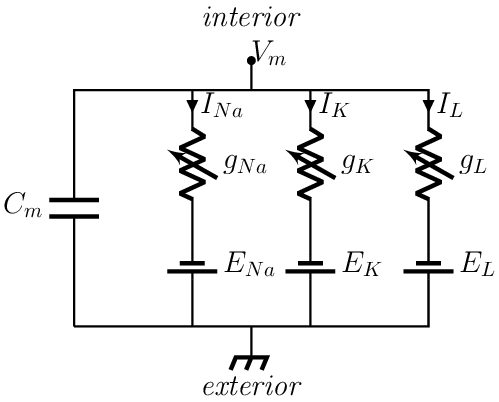
\includegraphics[scale=0.5]{../Figuras/circuito.png}
 \caption{Modelo de la membrana axónica modelada como circuito eléctrico, con los distintos canales presentes y su voltaje de reposo.}
 \label{fig:circuito1}
\end{figure}

Recordemos brevemente las definiciones de los dos tipos de canales protagonistas en el modelo:

\begin{definition}
 \emph{Canal persistente} Tiene un solo tipo de compuerta y dos estados posibles:
 \begin{enumerate}
  \item \textbf{Activado}
  \item \textbf{Desactivado}
 \end{enumerate}

\end{definition}

\begin{definition}
 \emph{Canal transitorio} Tiene compuertas de activación e inactivación, y tres estados:
 \begin{enumerate}
  \item \textbf{Activado} Ambas compuertas abiertas.
  \item \textbf{Desactivado} Compuerta de activación cerrada, inactivación abierta.
  \item \textbf{Inactivado} Compuerta de inactivación cerrada.
 \end{enumerate}

\end{definition}


Y retomando \hyperlink{LaEq}{la primera ecuación diferencial} donde tenemos, por un lado, la corriente que está pasando a través del capacitor, por otro lado, vamos a tener las corrientes que están circulando a través de los diferentes canales, 

\begin{equation}
  C_{m} \dfrac{dV_{m}}{dt} = - g_{Na} m^3 h(V_{m} - E_{Na}) - g_{K} n 4 (V_{m} - E_{K}) - g_{L} (V_{m} - E_{L}) + I_{ext}
  \tag{\ref{eq:corrientesEnLaMembrana2}}
\end{equation}

Las capacitancias y variables del lado izquierdo están explicadas en la sección \hyperlink{secc}{\emph{Modelo de la membrana como bicapa de lípidos}}, aquí vamos a retomar las ecuaciones \ref{eq:corrientesEnLaMembrana3},\ref{eq:corrientesEnLaMembrana4},\ref{eq:corrientesEnLaMembrana5} de esa misma sección, (recordemos que estás ecuaciones describen la probabilidad de que los canales iónicos estén abiertos) que son las siguientes:

\begin{equation}
  \dfrac{1}{\gamma(T)}\dfrac{dn}{dt} =  \alpha_{n^\infty} (V)(1 - n) - \beta_{n} (V) n = \dfrac{n(V)-n(t)}{\tau_{n}(V)}
  %\label{eq:probabilidades1}
  \tag{\ref{corrientesEnLaMembrana3}}
\end{equation}

\begin{equation}
  \dfrac{1}{\gamma(T)}\dfrac{dm}{dt} =  \alpha_{m} (V)(1 - m) - \beta_{m} (V) m = \dfrac{m^\infty(V)-m(t)}{\tau_{m}(V)}
  %\label{eq:probabilidades2}
  \tag{\ref{corrientesEnLaMembrana4}}
\end{equation}

\begin{equation}
  \dfrac{1}{\gamma(T)}\dfrac{dh}{dt} =  \alpha_{h} (V)(1 - h) - \beta_{h} (V) h = \dfrac{h^\infty(V)-h(t)}{\tau_{h}(V)}
  \tag{\ref{corrientesEnLaMembran53}}
\end{equation}

Ahora notemos los elementos en estas ecuaciones anteriores con \(ion\) pudiendo denotar las compuertas del potasio \(n\) o del sodio, ya sea \(m\) o \(h\):
\begin{itemize}
 \item \(\dfrac{1}{\gamma(T)}\) Este es el coeficiente de escala temporal, dependiente de la temperatura los por eso está apareciendo aquí una \(t\). Para las simulaciones que nosotros vamos a hacer vamos a pensar que estamos en una temperatura fija. 
 \item \(\alpha_{ion}(V)\) probabilidad de que una compuerta transite de cerrada a abierta.
 \item \(\beta_{ion}(V)\) probabilidad de que una compuerta transite de abierta a cerrada.
 \item \(ion^\infty(V)\) probabilidad de compuerta abierta en el equilibrio cuando \(t \rightarrow \infty\).
 \item \((ion)\) Probabilidad de que cada compuerta (n, m, h) esté abierta.
 \item \((1-ion)\) Probabilidad de que cada compuerta (n, m, h) esté cerrada.
 
 \item \(\tau_{ion}(V)\) Tiempo que toma llegar al equilibrio.
\end{itemize}


Lo que vamos a ver es que forma de escribir la ecuación depende precisamente del número de compuertas que tenían para poder abrirse y cerrarse. Reescribir la ecuación de esta manera lo que nos permite es medirlo en términos de estas probabilidades de que se abran y cierren las compuertas que serían 

Esta probabilidad se empieza a alterar conforme cambiamos el voltaje, pero no va a llegar a su valor de equilibrio sino hasta después de pasado un cierto periodo.


\section{Dinámica del voltaje durante un disparo} 

Ahora qué pasa cuando tomamos en cuenta que todas las compuertas están reaccionando al mismo tiempo.
Notemos primeramente como está reaccionando la membrana ante un impulso eléctrico o voltaje, en la siguiente imagen \ref{fig:voltaje1}.

\begin{figure}[h]
 \centering
 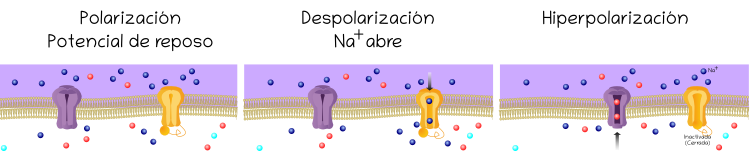
\includegraphics[scale=0.5]{../Figuras/polarizacion1.png}
 \caption{En la primera parte los canales están en un estado de reposo y la membrana está polarizada. En la segunda parte los canales han sido afectados por un impulso recibido desde el cono axónico, las compuertas de sodio se abren permitiendo el paso de iones de sodio al interior de la membrana y dejando a la membrana despolarizada. Momentos después la membrana llega a un estado de hiperpolarización donde intentará regresar al estado de equilibrio que tenía previamente, para esto la subpuerta de inactivación de sodio cerrará hasta no permitir el paso de sodio y el canal de potasio abrirá sus compuertas para dar salida a los potasios (iones positivos) que fluyan hacia el exterior de la membrana, así dejando el voltaje de la membrana incluso más negativo de lo que tenía durante su estado polarizado. }
 \label{fig:voltaje1}
\end{figure}

Ahora lo que vemos en la imagen \ref{fig:voltaje1} se gráfica de manera un poco más apegada a lo que pasa en los experimentos de la siguiente forma en la imagen \ref{fig:voltaje2}.

\begin{figure}[h]
 \centering
 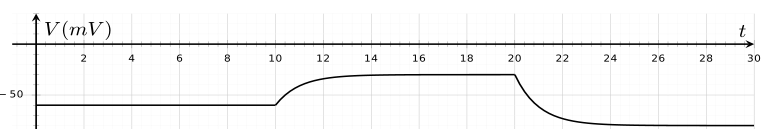
\includegraphics[scale=0.5]{../Figuras/polarizacion2.png}
 \caption{Gráfica del cambio de voltaje en la membrana dado un impulso atreves del tiempo. Cuando se rebasa el voltaje umbral, los canales de Na + y K + interactúan para producir una rápida despolarización de la membrana provocando una elevación del voltaje, para luego hiperpolarizarla. Durante el momento de despolarización la membrana puede llegar a valores positivos en este caso en particular el estímulo no es tan grande y se queda en valores negativos.}
 \label{fig:voltaje2}
\end{figure}


Ahora lo anterior está en términos de lo deseado, veamos entonces que paso en las mediciones de Hodgkin y Huxley con el axón en las siguientes gráficas \ref{fig:voltajeAB}, donde nos está mostrando como las subpuertas n y los factores \(\tau\), \(\alpha\) y \(\beta\) del canal de potasio se comportaron antes, durante y después del estímulo del voltaje. Recodemos que \emph{n} nos indica la probabilidad que las compuertas de potasio estén abiertas, este es un factor adimensional. \(\tau\) es el tiempo que tarda en llegar a un estado de equilibrio. \(\alpha\) y \(\beta\) las probabilidades que las compuertas del canal de potasio pasen de cerrados a abiertos y viceversa. 


Entonces notamos que en el mismo periodo de tiempo, la membrana está en reposo y conforme va recibiendo el voltaje incrementa la probabilidad que las compuestas de potasio estén abiertas, es decir \(n\) va incrementando conforme al estímulo, mientras que el estado de reposo es claramente alterado provocando que el valor \(\tau\) disminuya considerablemente. La probabilidad que las compuertas de potasio pasen de un estado cerrado a uno abierto durante el proceso (\(\alpha\)) aumenta prácticamente de forma exponencial, mientras que la probabilidad de que pasen de abierto a cerrado disminuye poco a poco. Con esto cumpliendo lo esperado en la dinámica del voltaje, al notar como está reaccionando el canal de potasio durante la polarización y despolarización (pulso). 



\begin{figure}[h]
 \centering
 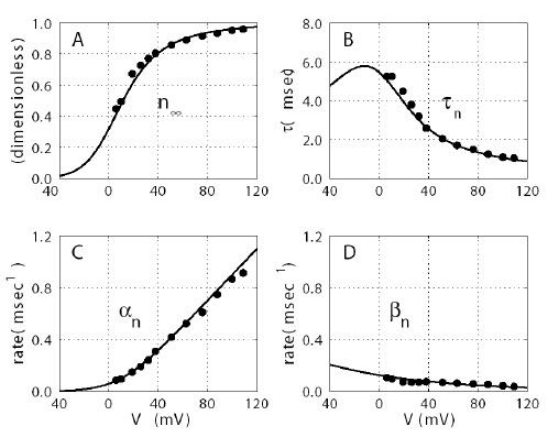
\includegraphics[scale=0.5]{../Figuras/medidasExperimentales.png}
 \caption{Medición experimental de los parámetros y ajuste manual de curvas. Imagen de Nelson 2004}
 \label{fig:voltajeAB}
\end{figure}

Con estas medidas experimentales ellos dan con curvas paramétricas ajustadas a los factores \(\alpha\) y \(\beta\) expresadas de la siguiente forma:

\begin{align*}
\alpha_{n}&=\dfrac{0.01(10-V)}{e^{\left(\dfrac{10-V}{10}\right)}-1}           &  \beta_{n}&=0.125e^{-\dfrac{V}{80}}\\
\alpha_{m}&=\dfrac{0.01(25-V)}{e^{\left(\dfrac{25-V}{10}\right)}-1}                    &  \beta_{m}&=4e^{-\dfrac{V}{18}}\\
\alpha_{h}&=0.07 e^{-\left(\dfrac{V}{20}\right)}              &  \beta_{h}&=\dfrac{1}{e^{\left(\dfrac{30-V}{10}\right)}+1}
\label{eq:curvas}
\end{align*}


Ahora veamos las gráficas de la dinámica del disparo pero ya con los las compuertas del potasio y sodio interactuando al mismo tiempo, en las figuras \ref{fig:voltajeActInac} y \ref{fig:voltajeActInac1}


\begin{figure}[h]
 \centering
 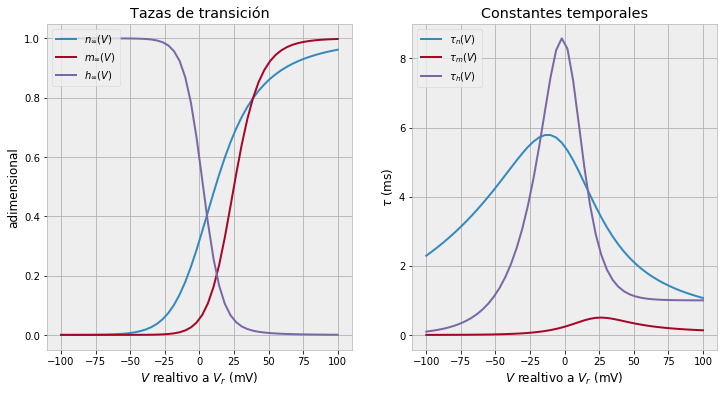
\includegraphics[scale=0.6]{../Figuras/actinac.png}
 %\caption{Activación e inactivación de los canales. Del lado izquierdo vemos que alrededor de los menos 50 mV aumenta la probabilidad que las compuertas de potasio abran y los potasios salgan, el sodio tarda un poco más en reaccionar para dejar entrar a los sodios, y la probabilidad que quede no bloqueado disminuye, hasta bloquear por completo a los iones de sodio alrededor de los 50 mV. Del lado derecho vemos como \(\tau\), va interactuando conforme al voltaje, el Na+ reacciona rápidamente ante él impuso pues regresa rápidamente a su estado de equilibrio, esto indica porque aún que el sodio abre sus compuertas, la compuerta de bloqueo se cierra rápidamente, dejando inactivado el canal, luego el K+ reacciona más lentamente para regresar a su estado de equilibrio dejando más tiempo activado el canal y salgan los potasios.}
 \label{fig:voltajeActInac}
\end{figure}


\begin{figure}[H]
 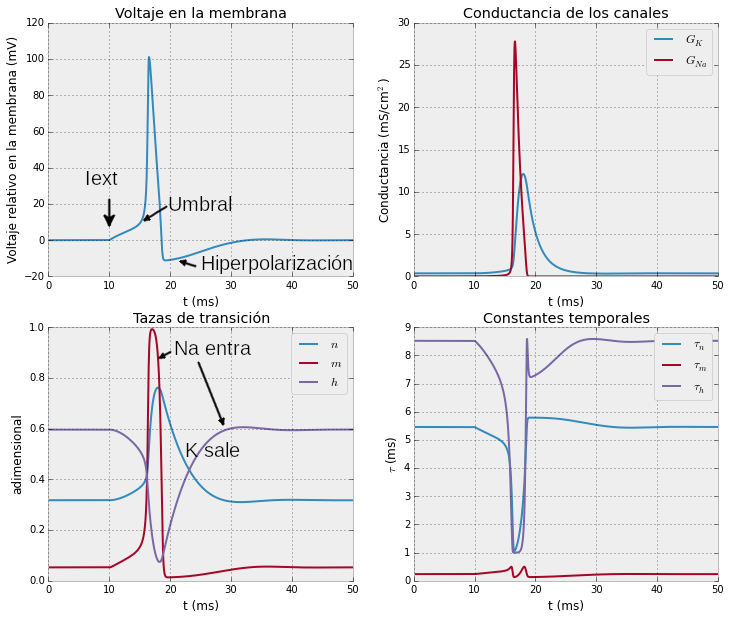
\includegraphics[scale=0.6]{../Figuras/disparo.png}
 \caption{Medidas experimentales del estímulo y la reacción de todos los componentes de la membrana. El origen en estás gráficas realmente esta representando el punto de equilibrio que es alrededor de los -70mV. Del lado superior izquierdo mostrando como cambia el voltaje de la membrana respecto al tiempo, del lado superior derecho el comportamiento de la conductancia de los canales mostrando que aunque la conductancia del sodio reacciona más, es más breve, mientras que el potasio reacciona en menor medida pero durante más tiempo. En la parte inferior derecha la taza de transición de las compuertas n,m y h, mostrando que en cuando llega el impulso el primero en reaccionar es el sodio permitiendo que entre muy brevemente el sodio e inactivandose casi inmediatamente después, mientras que en ese momento los potasios se están liberando hacia la parte exterior de la neurona. Finalmente del lado inferior izquierdo mostrando como se comporta las constantes temporales, mostrando que las compuertas de activación de sodio no son tan afectadas comparado a la compuerta de bloqueo, notando algunos cambio bruscos en esta, mientras que el potasio si se nota más afectado y durante más tiempo pero recuperándose sin cambios bruscos. }
 \label{fig:voltajeActInac1}
\end{figure}




\section{Simulación usando el método de Euler}

En esta sección se listará como estamos resolviendo las ecuaciones diferenciales, para tener una simulación numérica y se trata del algoritmo de integración \footnote{Hodgkin-Huxley Simulation Using Euler's Method lo puedes encontrar en la siguiente liga \url{https://webpages.uidaho.edu/rwells/techdocs/Biological\%20Signal\%20Processing/Chapter\%2003\%20The\%20Hodgkin-Huxley\%20Model.pdf}}. Las gráficas de la sección anterior se obtuvieron con el método de Euler que se describe más adelante.

\begin{algorithm}
  \caption{Algoritmo de integración de Euler [Wells pp51].}\label{AIE}
  \begin{algorithmic}[1]
    \Function{INTEGRADISPARO}{$T,\Delta T,V_{0},I_{ext}(t)$}
    \State Inicializar arreglos de longitud T: $T[],V[],n[],m[],h[],G_{Na}[],G_{K}[],\tau_{n}[],\tau_{m}[],\tau_{h}[] \gets arreglo[numeroDePasos] $
    \State  $V[0] \gets V_{0}$
    \For {$ t = 0  a  t = T cada \Delta t $}
        \State Calcular $\alpha_{n}, \beta_{n}, \alpha_{m}, \beta_{m},\alpha_{h}, \beta_{h} $ utilizando $V(t)$.
        \State Calcular las tres $\tau_{x} $ y $x^\infty $ apartir de las anteriores.
        \State Calcular las probabilidades de las compuertas $n, m, h, $ utilizando las ecuaciones en diferencias en su forma matricial $\Pi(t + \Delta t) = A_{\pi}\Pi(t) + B_{\pi}$.
        \State Calcular $G_{Na} = g_{Na}m^3h $ y $G_{K} = g_{K}n^4 $.
        \State Almacenar los resultados de este paso en los arreglos $T[], V[], n[], m[], h[], G_{Na}[], G_{K}[], \tau_{n}[], \tau_{m}[], \tau_{h}[] $
        \State $I_{ext} \gets I_{ext}(t) $
        \State Calcular $V_{m} (t + \Delta t) $
    \EndFor
    \State Devolver los arreglos $T[],V[],n[],m[],h[],G_{Na}[],G_{K}[],\tau_{n}[],\tau_{m}[],\tau_{h}[] $ con los resultados para los tiempos $[0,T] $
    \EndFunction
  \end{algorithmic}
\end{algorithm}


Comenzamos con un valor inicial y a partir de ahí empleamos las ecuaciones, para calcular las tangentes, aproximamos a la curva con su tangente.

Para la función \textproc{INTEGRADISPARO} necesitamos cuatro valores de entrada que van a provocar diferentes comportamientos:

\begin{enumerate}
 \item $T$ nos indica durante cuánto tiempo queremos correr la simulación.
 \item $\Delta T $ nos indica que tan finos queremos que sean los pasos recordemos que vamos a aproximar la función con segmentos de recta siguiendo la tangente. Si hacemos pasos demasiado pequeños nos vamos a tardar demasiado en hacer el cómputo.
 \item $V_{0} $ es el voltaje inicial en donde empieza nuestra simulación donde estaba en nuestra neurona cuando empezamos a trabajar.
 \item $I_{ext}(t) $ es la corriente externa, de qué magnitud fue el toque que le estamos dando en este momento al axón 

\end{enumerate}

A partir de los elementos iniciales proporcionados ya podemos calcular lo demás. Vamos a querer guardar lo que está ocurriendo para todos los tiempos desde cero hasta t en cada delta, y lo vamos a hacer en forma de arreglos donde en la posición [0], está la primera medición en t=0 y la posición t está la medición en el tiempo t. Vamos a tener toda una serie de puntos donde estamos guardando estos pasos para inicializarlo. 

Sabemos que necesitamos es un primer valor a partir del cual vamos a calcular la tangente y vamos a ir aproximando lo demás, entonces para eso queríamos \emph{el voltaje inicial}, como nosotros sabemos donde estaba en reposo nuestra célula originalmente, vamos a poder guardar ese voltaje como el primer valor para nuestra simulación. Ahora todos los demás elementos como $\alpha$s y $\beta$s y etc. se pueden calcular si ya conocíamos ese voltaje inicial, entonces a partir de este momento podemos repetir el mismo ciclo tantas veces como sea necesario para cubrir, el intervalo. 
Desde el tiempo inicial hasta el tiempo t, brincando de delta T en delta T. 
Entonces dado un voltaje vamos a calcular las diferentes \(\alpha\)s que son las que se medían experimentalmente originalmente utilizando las ecuaciones  de las curvas paramétricas ajustadas \ref{eq:curvas} (paso 5).

Ya calculadas las alfas y betas ahora si se puede calcular las $\tau$ , $n^{\infty}$, $m^{\infty}$, $h^{\infty}$ (paso 6).
Teniendo estas entonces podemos calcular las probabilidades para las compuertas n, m, h usando las ecuaciones en diferencias en forma matricial, estas matrices se pueden expresar como \ref{fig:matriX}.

\begin{figure}[H]
 \centering
 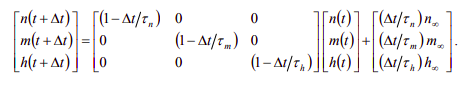
\includegraphics[scale=0.7]{../Figuras/matrix.png}
 \caption{Forma matricial para el cálculo de las probabilidades de las compuertas n, m, h.}
 \label{fig:matriX}
\end{figure}

Ahora esta parte fue importante sobre todo por el asunto de las pérdidas numéricas, recordemos que la computadora tiene una representación en punto flotante, lo cual quiere decir que un número real no se puede representar en la computadora, esto es importante por el problema del truncamiento, cada vez que se truncan dígitos al momento de calcular estamos perdiendo precisión, por esto es importante la forma en la que se procede a hacer los cálculos porque puede que se llegue a resultados un tanto distintos a los deseados aunque los cálculos sean correctos. 

Ya teniendo estos datos podemos fácilmente calcular las conductancias, simplemente sustituyendo los valores (paso 8).

Es bueno una vez que ya terminamos de calcular estos términos que se van a necesitar en la ecuación principal  \ref{eq:corrientesEnLaMembrana2} que es la del voltaje de la membrana,  ir almacenando en los \emph{resultados temporales} dentro de nuestros arreglos en la casilla que les corresponda, para ese momento (paso 8). En el paso 9, es donde ya vamos a utilizar \emph{la corriente externa} para meterla en la ecuación diferencial para el voltaje. Una vez que tengamos esto tenemos que repetirlo para cada paso, se está calculando el tiempo t,  entonces conforme avance el tiempo, va a dar el siguiente valor del voltaje, ya teniendo el siguiente valor del voltaje se va a poder usar para el siguiente paso ("como valor inicial nuevo") y así nos vamos a seguir todo el tiempo. 
Terminando el tiempo asignado a la simulación, tenemos ya los arreglos llenos de los datos que nos van a poder permitir graficar, qué fue lo que sucedió en cada tiempo, con cada canal y es precisamente  así que se puede graficar las mediciones presentadas en la sección anterior.
